\documentclass{article}
\usepackage[utf8]{inputenc}
\usepackage[left=1in,right=1in,top=1in,bottom=1in]{geometry}
\usepackage{crop,graphicx,array,color,flushend,stfloats,amsthm,chngpage,times,fancyhdr,lipsum,lastpage}

%%%%%%%%%%%%   Extra libraries & settings %%%%%%%%%%%%%
\setlength{\parskip}{0.25em}

%%%%%%%%%%%%   Header and Footer  %%%%%%%%%%%%%
\pagestyle{fancy}

\fancypagestyle{plain}{%
  \renewcommand{\headrulewidth}{0pt}%
  \fancyhf{}%
  \fancyfoot[R]{Page \bf\thepage\ \rm of \bf\pageref{LastPage}}%
}


%%%% Customise Titles and Headers: %%%%
\title{Don't forget adding title}
\author{Chinchuthakun Worameth (18B00033)}
\date{\today}

\fancyhf{}
\fancyhead[L]{Chinchuthakun Worameth}
\fancyhead[R]{18B00033}
\fancyfoot[R]{Page \bf\thepage\ \rm of \bf\pageref{LastPage}}


\AtBeginDocument{
%%%%%%%%%%%% Make Title and Format Lines %%%%%%%%%%%%
\maketitle											%
\vspace{-120px}										%
\noindent\rule{\linewidth}{1pt} \par				%
\vspace{100px}										%
\vspace{-20px}										%
\noindent\rule{\linewidth}{1pt} \par				%
\vspace{10px}										%
% %%%%%%%%%%%%%%%%%%% Content %%%%%%%%%%%%%%%%%%%%	
}

\AtEndDocument{
\bibliographystyle{IEEEtran}
\nocite{*}
\bibliography{citation}
}
% math stuff
\usepackage{amsmath}                % to use DeclareMathOperator
\usepackage{amssymb}
\usepackage{mathrsfs}
\usepackage{mathtools}
\usepackage{xargs}                  % for more than one optional arguments when define new commands
\usepackage{physics}                % vectors
\usepackage{mdframed}               % frames for definition, theorem, etc.
\usepackage[ruled]{algorithm2e}     % for algorithms
\usepackage{ifthen}                % for \ifthenelse
\usepackage{upgreek}

% figures and tables
\usepackage{titlesec}
\usepackage{caption}
\usepackage{subcaption}
\usepackage{multirow}
\usepackage{relsize}

% formatting some important single letters
\renewcommand{\epsilon}{\varepsilon}
\renewcommand{\phi}{\varphi}
\renewcommand{\upepsilon}{\upvarepsilon}
\renewcommand{\upphi}{\upvarphi}

% new operators
\DeclareMathOperator*{\argmin}{arg\,min}                % argmin
\DeclareMathOperator*{\argmax}{arg\,max}                % argmax
\DeclarePairedDelimiter\ceil{\lceil}{\rceil}            % ceiling function
\DeclarePairedDelimiter\floor{\lfloor}{\rfloor}         % floor function
\DeclarePairedDelimiter{\parens}{\lparen}{\rparen}      % parenthesis (use \parens* for automatically adjusting version)
\DeclarePairedDelimiter{\bracket}{[}{]}
\DeclarePairedDelimiter{\cbracket}{\{}{\}}
\DeclarePairedDelimiter{\ang}{\langle}{\rangle}
% \DeclarePairedDelimiter{\fourier}{\mathscr{F}\{}{\}}
% \DeclarePairedDelimiter{\invfourier}{\mathscr{F}^{-1}\{}{\}}

\newcommand{\fourier}[1]{\mathscr{F}\cbracket*{#1}}
\newcommand{\invfourier}[1]{\mathscr{F}^{-1}\cbracket*{#1}}
\newcommand {\dx}{\,dx}
\newcommand {\dy}{\,dy}
\newcommand {\dz}{\,dz}
\newcommand {\dt}{\,dt}
\newcommand {\du}{\,du}
\newcommand {\dtheta}{\,d\theta}
\newcommand {\domega}{\,d\omega}



\newcommand{\bigo}[1]{\ensuremath{\mathcal{O}\parens*{#1}}}
% new commands
\newcommand{\st}{such that }
\newcommand{\w}{where }
\newcommand{\del}{\nabla}
\newcommand{\larrow}{\leftarrow}
\newcommand{\rarrow}{\rightarrow}
\newcommand{\tbf}{\textbf}
\newcommand{\tit}{\textit}
\newcommand{\col}{\operatorname{col}}
\newcommand{\mat}[1]{\begin{matrix} #1 \end{matrix}}
% \newcommand{\vect}[1]{\boldsymbol{\mathbf{#1}}}
\newcommand{\vf}[1]{\boldsymbol{\mathbf{#1}}}
\newcommandx*{\seq}[2][1,2]{\ensuremath{#1, \ldots, #2}}
\newcommandx*{\ssum}[3][1,2,3]{\ensuremath{\sum_{#1 = #2}^{#3}}}
\newcommandx*{\sint}[2][1,2]{\ensuremath{\int_{#1}^{#2}}}
% \newcommandx*{\func}[4][1,2,3,4]{\ensuremath{#1^{\parens{#2}}_{#3}\parens{#4}}}
% \newcommandx*{\val}[3][1,2,3]{\ensuremath{#1^{\parens{#2}}_{#3}}}

% \newcommandx*{\func}[4][1=f,2=x,3,4, usedefault]{
%     \ifthenelse{\equal{#3}{}}{\ensuremath{#1_{#4}\parens{\vf{#2}}}}{\ensuremath{#1^{\parens{#3}}_{#4}\parens{\vf{#2}}}}
% }
\newcommandx*{\func}[3][1=f,2,3, usedefault]{
    \ifthenelse{\equal{#2}{}}{\ensuremath{#1_{#3}}}{\ensuremath{#1^{\parens{#2}}_{#3}}}
}
\newcommandx*{\val}[3][1,2,3, usedefault]{
    \ifthenelse{\equal{#2}{}}{\ensuremath{\vf{#1}_{#3}}}{\ensuremath{\vf{#1}^{\parens{#2}}_{#3}}}
}

\newcommandx*{\Real}[1][1, usedefault]{\ensuremath{\mathbb{R}^{#1}}}                % set of real number
\newcommandx*{\Int}[1][1, usedefault]{\ensuremath{\mathbb{Z}^{#1}}}                 % set of integer
\newcommandx*{\Natural}[1][1, usedefault]{\ensuremath{\mathbb{N}^{#1}}}             % set of natural number
\newcommandx*{\normal}[2][1=0, 2=1, usedefault=!]{\ensuremath{\mathcal{N}(#1,#2)}}  % Gaussian distribution

% define frame environment
% \newmdtheoremenv{definition}{Definition}
% \newmdtheoremenv{proposition}{Proposition}
% \newmdtheoremenv{corollary}{Corollary}
% \newmdtheoremenv{lemma}{Lemma}
% \newmdtheoremenv{theorem}{Theorem}
% \newmdtheoremenv{remark}{Remark}

% define keywords for algorithm
\SetKwInOut{Input}{Input}
\SetKwInOut{Output}{Output}
\SetKwInOut{Parameter}{Parameter}

% \begin{theorem}{text}{label}
% refer as \ref{tha:label}
\usepackage{tcolorbox}
\tcbuselibrary{theorems,breakable} %% を読み込む
\definecolor{burgundy}{rgb}{0.5, 0.0, 0.13}
\newtcbtheorem[number within=section]{theorem}{Theorem}%
{colframe=burgundy,colback=burgundy!2!white,
rightrule=0pt,leftrule=0pt,bottomrule=2pt,
colbacktitle=burgundy,theorem style=standard,breakable,arc=0pt}{theo}

\definecolor{oxfordblue}{rgb}{0.0, 0.13, 0.28}
\newtcbtheorem[number within=section]{definition}{Definition}%
{colframe=oxfordblue,colback=oxfordblue!2!white,
rightrule=0pt,leftrule=0pt,bottomrule=2pt,
colbacktitle=oxfordblue,theorem style=standard,breakable,arc=0pt}{def}

\definecolor{cadmiumorange}{rgb}{0.93, 0.53, 0.18}
\newtcbtheorem[number within=section]{remark}{Remark}%
{colframe=cadmiumorange,colback=cadmiumorange!2!white,
rightrule=0pt,leftrule=0pt,bottomrule=2pt,
colbacktitle=cadmiumorange,theorem style=standard,breakable,arc=0pt}{rem}

% equation numbering
\numberwithin{equation}{section}

%%%%%%%%%%%%%%%%%%%%%%%%%%%
\usepackage{listings}
\usepackage{xcolor}

\definecolor{codegreen}{rgb}{0,0.6,0}
\definecolor{codegray}{rgb}{0.5,0.5,0.5}
\definecolor{codepurple}{rgb}{0.58,0,0.82}
\definecolor{backcolour}{rgb}{0.95,0.95,0.92}

\lstdefinestyle{mystyle}{
    backgroundcolor=\color{backcolour},   
    commentstyle=\color{codegreen},
    keywordstyle=\color{magenta},
    numberstyle=\tiny\color{codegray},
    stringstyle=\color{codepurple},
    basicstyle=\ttfamily\footnotesize,
    breakatwhitespace=false,         
    breaklines=true,                 
    captionpos=b,                    
    keepspaces=true,                 
    numbers=left,                    
    numbersep=5pt,                  
    showspaces=false,                
    showstringspaces=false,
    showtabs=false,                  
    tabsize=2
}

\lstset{style=mystyle}

\makeatletter
\renewcommand*\env@matrix[1][\arraystretch]{%
  \edef\arraystretch{#1}%
  \hskip -\arraycolsep
  \let\@ifnextchar\new@ifnextchar
  \array{*\c@MaxMatrixCols c}}
\makeatother
\title{Computer Graphics Assignment \#1}
\begin{document}

\section{Question}
Answer the inverse Fourier transform of the functions:
$$
\begin{gathered}
    \func[F][][1](\omega_x,\omega_y) = \func[\delta](\omega_x - \sqrt{3})\func[\delta](\omega_y - 1) + \func[\delta](\omega_x + \sqrt{3})\func[\delta](\omega_y + 1) \\
    \func[F][][2](\omega_x,\omega_y) = i\func[\delta](\omega_x - \sqrt{3})\func[\delta](\omega_y - 1) - i\func[\delta](\omega_x + \sqrt{3})\func[\delta](\omega_y + 1)
\end{gathered}
$$

\section{Answer}
\subsection{Equation}
\subsubsection{Inverse Fourier transform of $\func[F][][1]$}

\begin{align}
\invfourier{\func[F][][1](\omega_x,\omega_y)} 
&= \invfourier{\func[\delta](\omega_x - \sqrt{3})\func[\delta](\omega_y - 1) + \func[\delta](\omega_x + \sqrt{3})\func[\delta](\omega_y + 1)} \\
&= \invfourier{\func[\delta](\omega_x - \sqrt{3})\func[\delta](\omega_y - 1)} + \invfourier{\func[\delta](\omega_x + \sqrt{3})\func[\delta](\omega_y + 1)}
\end{align}
By applying the property of the dirac delta function $\sint[-\infty][\infty] \func[f](x)\func[\delta](x - x_0) \dx = \func[f](x_0)$, we have
\begin{align}
\invfourier{\func[\delta](\omega_x - \sqrt{3})\func[\delta](\omega_y - 1)}
&= \frac{1}{4\pi^2} \sint[-\infty][\infty]  \func[\delta](\omega_y - 1) e^{i\omega_y y} \sint[-\infty][\infty] \func[\delta](\omega_x - \sqrt{3}) e^{i\omega_x x} \domega_x  \domega_y \\
&= \frac{1}{4\pi^2} \sint[-\infty][\infty]  \func[\delta](\omega_y - 1) e^{i\omega_y y} \parens*{e^{\sqrt{3} ix}}  \domega_y \\
&= \frac{1}{4\pi^2} \parens*{e^{\sqrt{3} ix}} \parens*{e^{iy}} \label{first-term}
\end{align}
and similarly,
\begin{equation}
    \invfourier{\func[\delta](\omega_x + \sqrt{3})\func[\delta](\omega_y + 1)} = \frac{1}{4\pi^2} \parens*{e^{-\sqrt{3} ix}} \parens*{e^{-iy}} \label{second-term}
\end{equation}
Therefore, by combining result from \eqref{first-term} and \eqref{second-term} and applying the Euler's formula, we have
\begin{align}
\invfourier{\func[F][][1](\omega_x,\omega_y)} 
&= \frac{1}{4\pi^2} \parens*{{e^{\sqrt{3} ix + iy}} + {e^{-\sqrt{3} ix - iy}}} \label{combine} \\
&= \frac{1}{4\pi^2} \parens*{\cos(\sqrt{3}x + y) + i\sin(\sqrt{3}x + y) + \cos(-\sqrt{3}x - y) + i\sin(-\sqrt{3}x - y)} \\
&= \frac{1}{4\pi^2} \parens*{\cos(\sqrt{3}x + y) + i\sin(\sqrt{3}x + y) + \cos(\sqrt{3}x + y) - i\sin(\sqrt{3}x + y)} \\
&= \frac{1}{2\pi^2} \cos(\sqrt{3}x + y) \label{result-1}
\end{align}

\subsubsection{Inverse Fourier transform of $\func[F][][2]$}

Since $\func[F][][1]$ and $\func[F][][2]$ are the same, except the coefficient $i$ and the minus sign in the latter, we can modify the expression in \eqref{combine}:
\begin{align}
\invfourier{\func[F][][2](\omega_x,\omega_y)} 
&= \frac{i}{4\pi^2} \parens*{{e^{\sqrt{3} ix + iy}} - {e^{-\sqrt{3} ix - iy}}} \\
&= \frac{i}{4\pi^2} \parens*{\cos(\sqrt{3}x + y) + i\sin(\sqrt{3}x + y) - \cos(-\sqrt{3}x - y) - i\sin(-\sqrt{3}x - y)} \\
&= \frac{i}{4\pi^2} \parens*{\cos(\sqrt{3}x + y) + i\sin(\sqrt{3}x + y) - \cos(\sqrt{3}x + y) + i\sin(\sqrt{3}x + y)} \\
&= -\frac{1}{2\pi^2} \sin(\sqrt{3}x + y) \label{result-2}
\end{align}

\subsection{Graph}
We can visualize the inverse Fourier transform of $\func[F][][1]$ and $\func[F][][2]$, described in \eqref{result-1} and \eqref{result-2}, by using Python.

\begin{figure}[h]
    \centering
    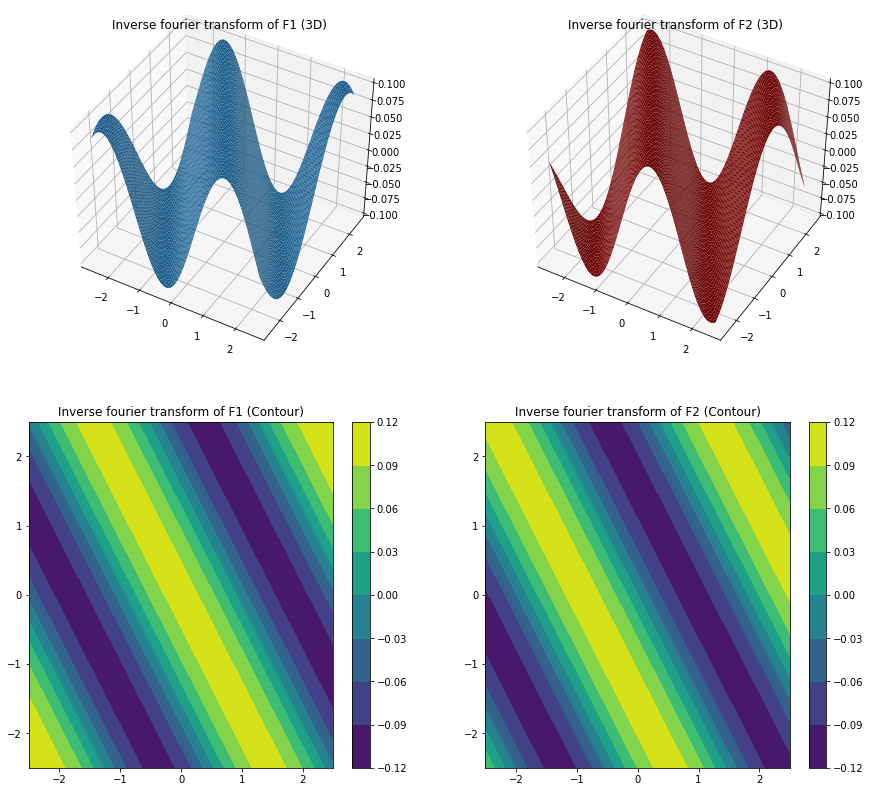
\includegraphics[width=0.9\textwidth]{figures/assignment1/cg1-assignment1.png}
    \caption{Visualization of $\invfourier{\func[F][][1](\omega_x,\omega_y)}$ and $\invfourier{\func[F][][2](\omega_x,\omega_y)}$}
\end{figure}

\subsection{Text (Full sentences)}
\begin{itemize}
    \item $\invfourier{\func[F][][1](\omega_x,\omega_y)}$ is a cosine function with an amplitude of $\frac{1}{2\pi}$ in the direction of 30 degrees from $x$-axis. Its period is $\parens*{\frac{2\pi}{\sqrt{3}}, 2\pi}$.
    \item Similarly, $\invfourier{\func[F][][2](\omega_x,\omega_y)}$ is a sine function with an amplitude of $\frac{1}{2\pi}$ in the direction of 30 degrees from $x$-axis. Its period is $\parens*{\frac{2\pi}{\sqrt{3}}, 2\pi}$. It is also reflected over the unit vector $\parens*{\sqrt{3}, 1}$.
\end{itemize}

\end{document}